\section{El grupo SG14}

\begin{frame}[t]{C++ y videojuegos}
\begin{columns}

\column{.6\textwidth}
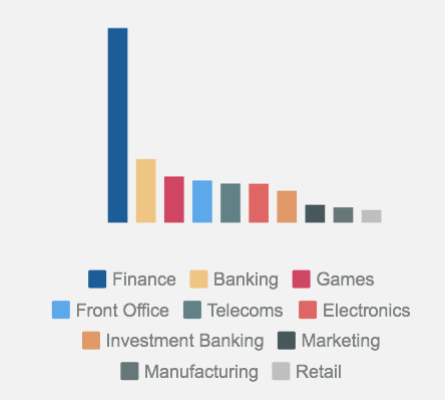
\includegraphics[height=.7\textheight]{figs/clion-market}

\column{.4\textwidth}

\includegraphics[width=4cm]{logos/clion}


\includegraphics[width=4cm]{logos/jetbrains}

\end{columns}
\vfill
{\tiny\color{blue}\textbf{\url{http://blog.jetbrains.com/clion/2015/07/infographics-cpp-facts-before-clion/}}}
\end{frame}

\begin{frame}{El comité de C++}
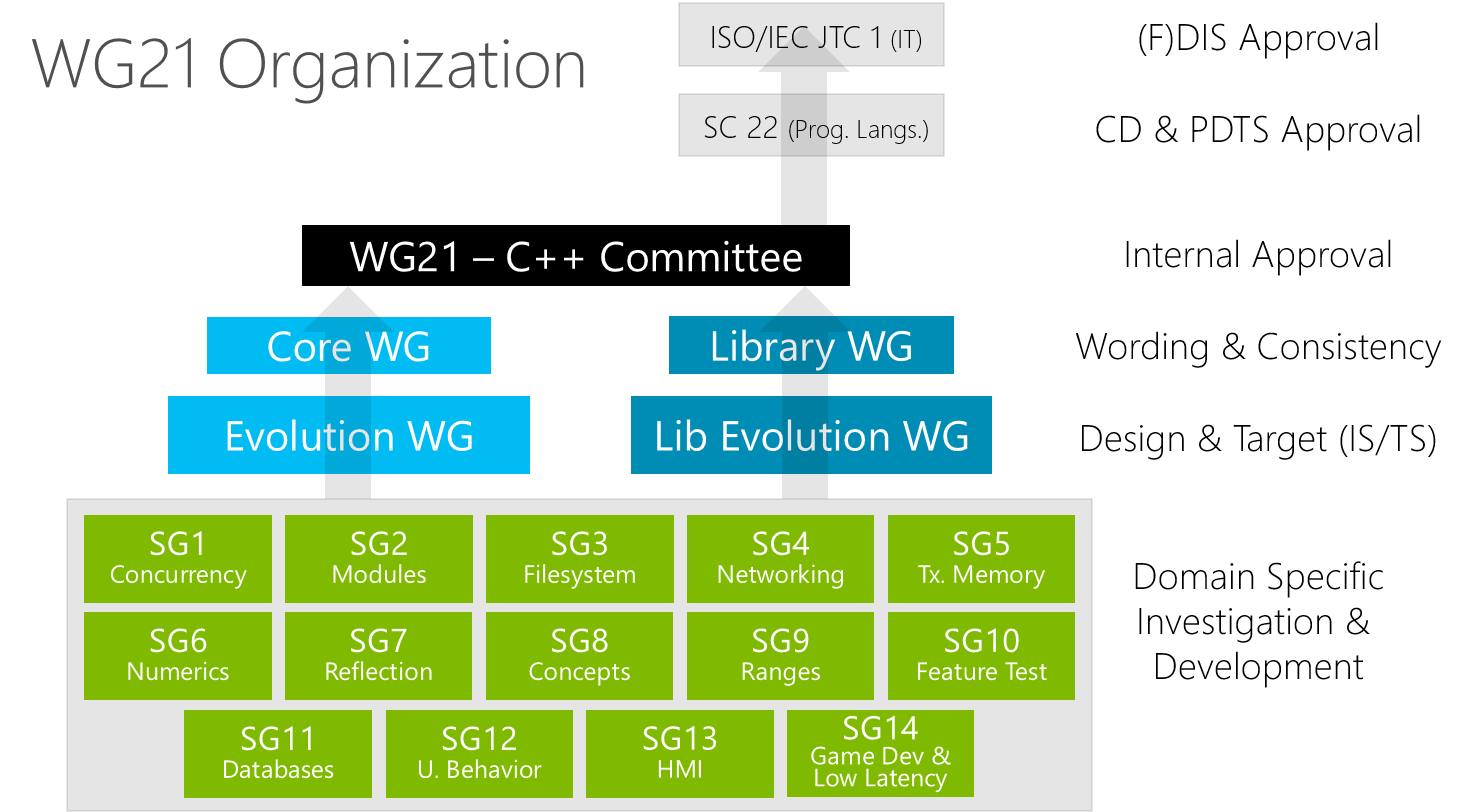
\includegraphics[height=6cm]{figs/sc22-wg21}
\end{frame}

\begin{frame}[t]{Orígenes}
\begin{itemize}
  \item \textbf{CppCon 2014}: Comité se encuentra con desarrolladores.
    \begin{itemize}
      \item Discusiones preliminares.
      \item Lista de correo y grupo en Google Groups.
      \item N4456: Towards improved support for games, graphics, real-time, low latency, embedded systems.
    \end{itemize}
  \vfill\pause
  \item Creación de SG14: \emph{Game Development and Low Latency}
    \begin{itemize}
      \item Chair: Michael Wong (IBM).
      \item Próxima reunión: GDC 2016.
      \item SG14 se reune para enviar propuestas a WG21 (Comité C++).
    \end{itemize}
\end{itemize}
\end{frame}

\begin{frame}[t,shrink=10]{Otros sectores interesados}
\begin{itemize}
  \item Otros sectores atraidos:
    \begin{itemize}
      \item Finnancial/Trading.
      \item Banca.
      \item Simulación.
      \item HPC.
      \item Big Data Analytics?
    \end{itemize}
  \vfill\pause
  \item ¿Por qué?
    \begin{itemize}
      \item Simulaciones interactivas 
        \begin{itemize}
          \item Simulación, software de formación.
        \end{itemize}
      \item Gráficos en tiempo real.
        \begin{itemize}
          \item Simulación, software de formación.
        \end{itemize}
      \item Computación de baja latencia .
        \begin{itemize}
          \item Simulación, software de formación, finanzas, trading.
        \end{itemize}
      \item Recursos restringidos. 
        \begin{itemize}
          \item Sistemas empotrados.
        \end{itemize}
      \item Altas prestaciones 
        \begin{itemize}
          \item Computación científica, Big Data analytics.
        \end{itemize}
    \end{itemize}
\end{itemize}
\end{frame}
